\subsection{KENN with multiloss function}
In previous experiments, it has been observed that the pre-KENN network adapts to the presence of KENN regardless of the parameters configuration. From these results comes the intuition to make the pre-KENN network more independent, with the purpose of exploiting the logical knowledge more effectively. To achieve this, the idea is to define a custom multiloss function to simultaneously improve the quality of the pre-KENN and post-KENN predictions.

%\subsubsection{Multiloss function}
The proposed multiloss function is computed by combining the Binary Cross-Entropy (BCE) loss values obtained from the pre-KENN and post-KENN preactivations. To make it possible, the model has been adapted to provide two outputs: one before and one after KENN's layer. The goal is to optimize the post-KENN predictions while preserving a discrete quality of pre-KENN predictions. The final loss is computed by the convex combination of the two losses whose influences are regulated by the parameter $ \alpha $. The resulting formula is the following:

% \begin{gather*}
%     L(y_{pred},y_{true}) = \alpha \cdot BCE(y_{prekenn}, y_{true}) + (1 - \alpha) \cdot BCE(y_{postkenn}, y_{true})
% \end{gather*}

\begin{gather*}
    L(Y, Y', Y_{t}) = \alpha \cdot BCE(Y, Y_{t}) + (1 - \alpha) \cdot BCE(Y', Y_{t})
\end{gather*}
where $Y$ denotes the pre-KENN predictions, $Y'$ the post-KENN predictions, and $Y_{t}$ the values of the ground truth.


\subsubsection{Setup}
The models involved in this experiment are trained following the \textit{Setup B}. The configuration of the other parameters is the following:
\begin{itemize}
    \item \textbf{KB modes:} Bottom Up and Top Down
    \item \textbf{initial clause weights:} 0.5 and variable\footnote{With the term ``variable" we mean that each clause can be initialized with a different value. The original implementation of KENN did not contemplate this possibility when setting clause weights as learnable parameters, so we introduced a small modification to make it possible.}
    \item \textbf{learnable clause weights}
    \item \textbf{encoder:} DistilBERT and BERT, with adapters
    \item \textbf{loss function:} multiloss with $\alpha = 0.5$
\end{itemize}
The total number of configurations obtained by varying these parameters is 8. Since the pre-KENN network is expected to be less influenced by KENN, the clause weights are set as learnable parameters with small initial values to start with a soft influence and let the network establish the relevance of each clause. Indeed, the choice of learnable clause weights allows us to study the weight evolution during the epochs and determine which are the most useful and the least useful clauses. Furthermore, for each clause, the types that are the antecedents of an implication rule (i.e., the types that propagate the information and uniquely characterize the used KBs) have been studied to look for some recurring behavioral patterns. The \textit{Hybrid} mode is excluded from this study because it involves the same clauses of \textit{Bottom Up} and \textit{Top Down}, but with the addition of noise due to the presence of conflicts. For this reason, it would not have been possible to carry out an accurate analysis.

\subsubsection{Results on FIGER}
\paragraph{DistilBERT}
The results obtained using DistilBERT as encoder show some very interesting behaviors of the clause weights. Starting from the Bottom Up, if we look at the distribution of final clause weights in Figure~\ref{fig:weight_distrib_distilbert_figer_bu_multiloss} we can see that almost every weight decreases its initial value. This attitude is not observable in Figure~\ref{fig:weight_distrib_distilbert_figer_bu_learnable} when using KENN with a standard loss and learnable weights. If we look at the figure, we can see widely different results since almost every weight increases its starting value. The same trend is detectable in the Top Down mode, as shown in Figure~\ref{fig:weight_distrib_distilbert_figer_td}.

\begin{figure}[bth]
     \centering
     \begin{subfigure}[b]{0.45\textwidth}
         \centering
         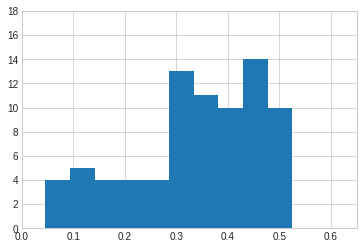
\includegraphics[width=\textwidth]{figures/weight_distrib_distilbert_figer_bu_multiloss.png}
         \caption{Multiloss model - Epoch 55 (563K examples)}
         \label{fig:weight_distrib_distilbert_figer_bu_multiloss}
     \end{subfigure}
     \hspace{10px}
     \begin{subfigure}[b]{0.45\textwidth}
         \centering
         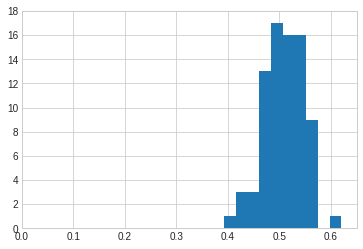
\includegraphics[width=\textwidth]{figures/weight_distrib_distilbert_figer_bu_learnable.png}
         \caption{Standard loss model - Epoch 42 (430K examples)}
         \label{fig:weight_distrib_distilbert_figer_bu_learnable}
     \end{subfigure}
    \caption{Distributions of the final learned clause weights for the Bottom Up KB mode using DistilBERT-based models - FIGER}
    \label{fig:weight_distrib_distilbert_figer_bu}
\end{figure}

\begin{figure}[bth]
     \centering
     \begin{subfigure}[b]{0.45\textwidth}
         \centering
         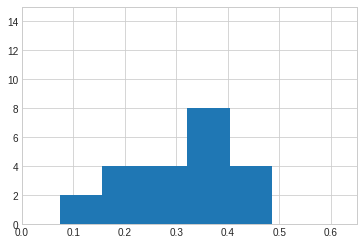
\includegraphics[width=\textwidth]{figures/weight_distrib_distilbert_figer_td_multiloss.png}
         \caption{Multiloss model - Epoch 42 (430K examples)}
         \label{fig:weight_distrib_distilbert_figer_td_multiloss}
     \end{subfigure}
     \hspace{10px}
     \begin{subfigure}[b]{0.45\textwidth}
         \centering
         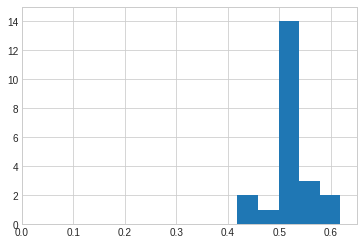
\includegraphics[width=\textwidth]{figures/weight_distrib_distilbert_figer_td_learnable.png}
         \caption{Standard loss model - Epoch 39 (399K examples)}
         \label{fig:weight_distrib_distilbert_figer_td_learnable}
     \end{subfigure}
    \caption{Distributions of the final learned clause weights for the Top Down KB mode using DistilBERT-based models - FIGER}
    \label{fig:weight_distrib_distilbert_figer_td}
\end{figure}


Moving on to the analysis of the types involved in the clauses we can observe an unexpected behavior. For both Bottom Up and Top Down modes, this study intercepts a remarkable fact: the more a type occurs in the training set, the lower the final weight of its clause. The few clauses that preserve a high weight are those whose antecedents are the rarest in the dataset. Starting from the Bottom Up mode, we can see in Figure~\ref{fig:weight_freq_distilbert_figer_bu_multiloss} a graph showing the relation between the final weight and the frequency of each type S. Looking at the figure, we can clearly observe that there is a strong correlation between weight and frequency. Indeed, the correlation coefficient is -0.77. The Top Down mode (Figure~\ref{fig:weight_freq_distilbert_figer_td_multiloss}) also presents a negative correlation, this time of -0.68 with respect to the frequencies of types F.
%This behavior may be explained by the fact that KENN introduces too much noise to types that the network can already predict discretely without the use of knowledge. 

\begin{figure}[bth]
     \centering
     \begin{subfigure}[b]{0.7\textwidth}
         \centering
         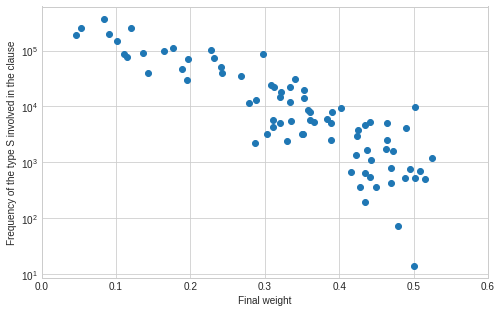
\includegraphics[width=\textwidth]{figures/weight_freq_distilbert_figer_bu_multiloss.png}
         \caption{Bottom Up - Epoch 55 (563K examples)}
         \label{fig:weight_freq_distilbert_figer_bu_multiloss}
         \vspace{10px}
     \end{subfigure}
     \begin{subfigure}[b]{0.7\textwidth}
         \centering
         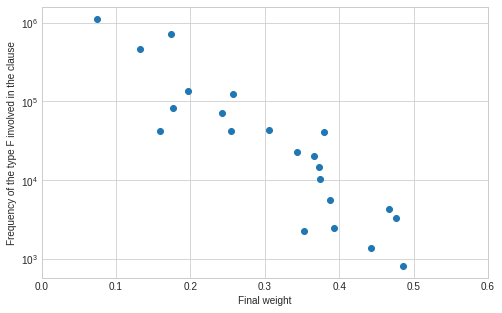
\includegraphics[width=\textwidth]{figures/weight_freq_distilbert_figer_td_multiloss.png}
         \caption{Top Down - Epoch 42 (430K examples)}
         \label{fig:weight_freq_distilbert_figer_td_multiloss}
     \end{subfigure}
    \caption{Relation between types frequency (log scale) and final clause weights of multiloss models using DistilBERT - FIGER}
    \label{fig:weight_freq_distilbert_figer}
\end{figure}

By inspecting the weight evolution over the epochs, it emerged that the clause weights keep decreasing until the last epoch, but it is not known for how long they would have continued. To observe in advance the effect of higher epochs and see if some clauses would have reached a weight close to zero, new models were trained starting from variable weights assigned with respect to the frequency of the antecedents of each clause. Clauses involving popular types were assigned a weight of 0.2, while the others kept a weight of 0.5. The weight assignment is based on a frequency threshold of 70K for Bottom Up and 50K for Top Down\footnote{the values are chosen by observing the graphs, without formalizing a mathematical criterion}. The results of these runs are shown in Figure~\ref{fig:weight_freq_distilbert_figer_bu_multiloss_variable} and Figure~\ref{fig:weight_freq_distilbert_figer_td_multiloss_variable} for Bottom Up and Top Down, respectively. As we can see, most clause weights decreased their values even when starting from lower initial values.
%However, by analyzing the weight evolution, it emerged that their decrease over the epochs was slowed down. The reason for this fact is that clauses now have less influence on the final prediction, so they are penalized in a minor way by the loss function.

\begin{figure}[bth]
     \centering
     \begin{subfigure}[b]{0.7\textwidth}
         \centering
         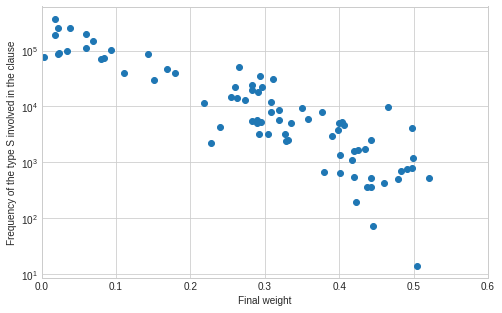
\includegraphics[width=\textwidth]{figures/weight_freq_distilbert_figer_bu_multiloss_variable.png}
         \caption{Bottom Up - Epoch 71 (727K examples)}
         \label{fig:weight_freq_distilbert_figer_bu_multiloss_variable}
         \vspace{10px}
     \end{subfigure}
     \begin{subfigure}[b]{0.7\textwidth}
         \centering
         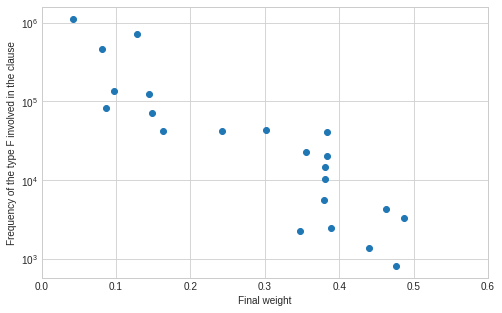
\includegraphics[width=\textwidth]{figures/weight_freq_distilbert_figer_td_multiloss_variable.png}
         \caption{Top Down - Epoch 42 (430K examples)}
         \label{fig:weight_freq_distilbert_figer_td_multiloss_variable}
     \end{subfigure}
    \caption{Relation between types frequency (log scale) and final clause weights of multiloss models using DistilBERT and \textit{variable} clause weights - FIGER}
    \label{fig:weight_freq_distilbert_figer_variable}
\end{figure}

\paragraph{BERT}
The experiments performed using BERT showed an identical behavior. The results obtained with weights set to 0.5 for every clause are shown in Figure~\ref{fig:weight_freq_bert_figer}. The correlation between weight and frequency is similar (-0.76 in Bottom Up, -0.74 in Top Down) as well as the weight evolution during the epochs. The only difference with respect to DistilBERT is that BERT needs fewer epochs to converge, so its weights have decreased less as it performed fewer backward propagation operations. Much lower weights are reached when using the setup with variable weights as reported in Figure~\ref{fig:weight_freq_bert_figer_variable}.

\begin{figure}[bth]
     \centering
     \begin{subfigure}[b]{0.7\textwidth}
         \centering
         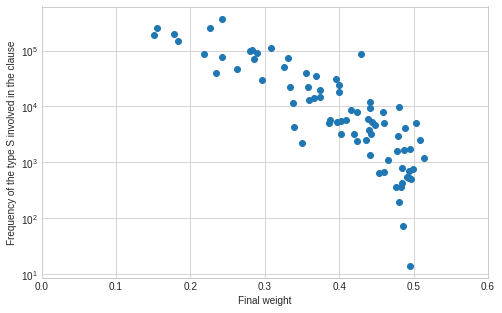
\includegraphics[width=\textwidth]{figures/weight_freq_bert_figer_bu_multiloss.png}
         \caption{Bottom Up - Epoch 35 (358K training examples)}
         \label{fig:weight_freq_bert_figer_bu_multiloss}
         \vspace{10px}
     \end{subfigure}
     \begin{subfigure}[b]{0.7\textwidth}
         \centering
         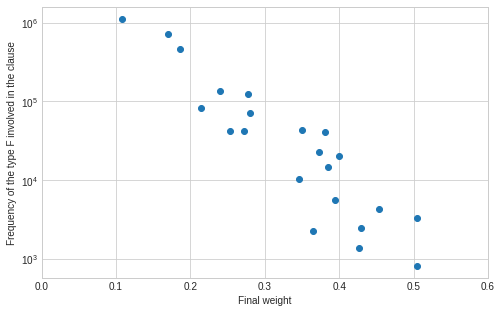
\includegraphics[width=\textwidth]{figures/weight_freq_bert_figer_td_multiloss.png}
         \caption{Top Down - Epoch 35 (358K training examples)}
         \label{fig:weight_freq_bert_figer_td_multiloss}
     \end{subfigure}
    \caption{Relation between types frequency (log scale) and final clause weights of multiloss models using BERT - FIGER}
    \label{fig:weight_freq_bert_figer}
\end{figure}

\begin{figure}[bth]
     \centering
     \begin{subfigure}[b]{0.7\textwidth}
         \centering
         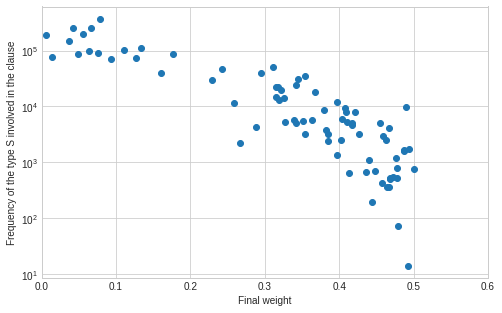
\includegraphics[width=\textwidth]{figures/weight_freq_bert_figer_bu_multiloss_variable.png}
         \caption{Bottom Up - Epoch 49 (501K training examples)}
         \label{fig:weight_freq_bert_figer_bu_multiloss_variable}
         \vspace{10px}
     \end{subfigure}
     \begin{subfigure}[b]{0.7\textwidth}
         \centering
         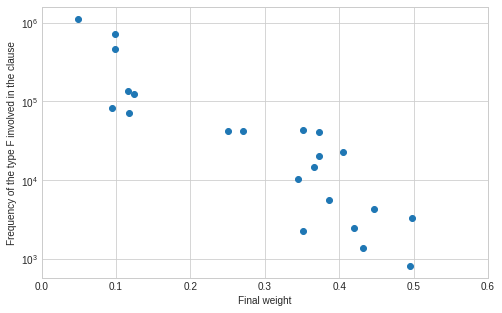
\includegraphics[width=\textwidth]{figures/weight_freq_bert_figer_td_multiloss_variable.png}
         \caption{Top Down - Epoch 33 (337K training examples)}
         \label{fig:weight_freq_bert_figer_td_multiloss_variable}
     \end{subfigure}
    \caption{Relation between types frequency (log scale) and final clause weights of multiloss models using BERT and \textit{variable} clause weights - FIGER}
    \label{fig:weight_freq_bert_figer_variable}
\end{figure}


\subsubsection{Results on BBN}
The experiments on BBN were performed directly on BERT. In Figure~\ref{fig:weight_freq_bert_bbn} are represented the graphs of weights and frequencies using the same weight for each clause. The correlation coefficients of the Bottom Up and Top Down modes are -0.73 and -0.55, respectively. The results obtained after repeating the experiments using variable weights are shown in Figure~\ref{fig:weight_freq_bert_bbn_variable}. The weight assignment is based on a frequency threshold of 1700 for Bottom Up and 1500 for Top Down\footnote{the values are chosen by observing the graphs, without formalizing a mathematical criterion}. Looking at the graphs, it is possible to observe that most of the weights continued to decrease.

\begin{figure}
     \centering
     \begin{subfigure}[b]{0.7\textwidth}
         \centering
         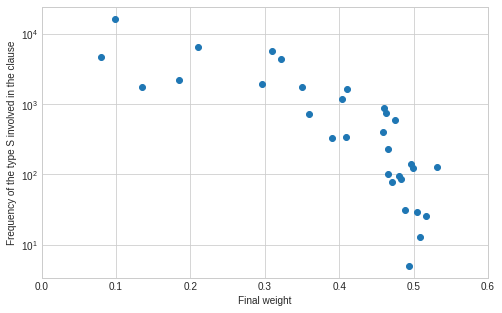
\includegraphics[width=\textwidth]{figures/weight_freq_bert_bbn_bu_multiloss.png}
         \caption{Bottom Up - Epoch 28 (286K training examples)}
         \label{fig:weight_freq_bert_bbn_bu_multiloss}
         \vspace{10px}
     \end{subfigure}
     \begin{subfigure}[b]{0.7\textwidth}
         \centering
         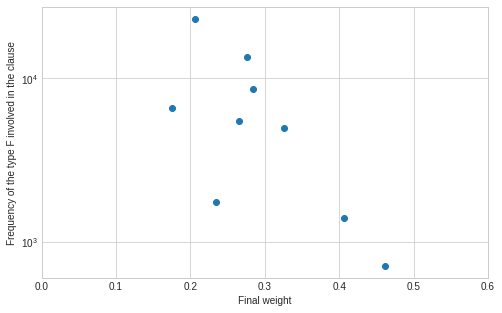
\includegraphics[width=\textwidth]{figures/weight_freq_bert_bbn_td_multiloss.png}
         \caption{Top Down - Epoch 19 (194K training examples)}
         \label{fig:weight_freq_bert_bbn_td_multiloss}
     \end{subfigure}
    \caption{Relation between types frequency (log scale) and final clause weights of multiloss models using BERT - BBN}
    \label{fig:weight_freq_bert_bbn}
\end{figure}

\begin{figure}
     \centering
     \begin{subfigure}[b]{0.7\textwidth}
         \centering
         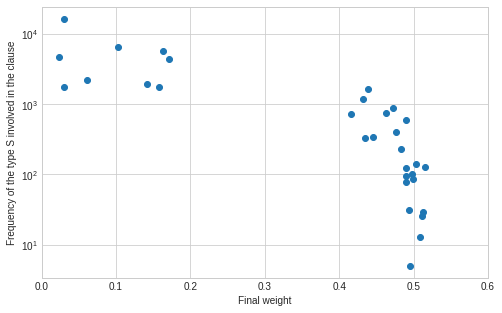
\includegraphics[width=\textwidth]{figures/weight_freq_bert_bbn_bu_multiloss_variable.png}
         \caption{Bottom Up - Epoch 19 (194K training examples)}
         \label{fig:weight_freq_bert_bbn_bu_multiloss_variable}
         \vspace{10px}
     \end{subfigure}
     \begin{subfigure}[b]{0.7\textwidth}
         \centering
         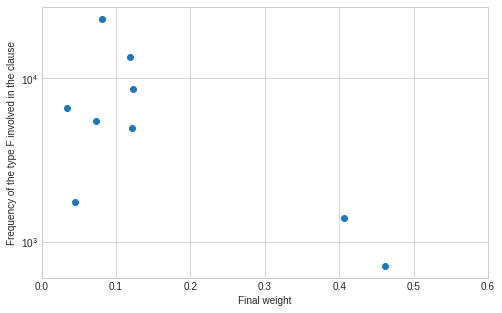
\includegraphics[width=\textwidth]{figures/weight_freq_bert_bbn_td_multiloss_variable.png}
         \caption{Top Down - Epoch 19 (194K training examples)}
         \label{fig:weight_freq_bert_bbn_td_multiloss_variable}
     \end{subfigure}
    \caption{Relation between types frequency (log scale) and final clause weights of multiloss models using BERT and \textit{variable} clause weights - BBN}
    \label{fig:weight_freq_bert_bbn_variable}
\end{figure}



\subsubsection{Conclusion}
The multiloss experiments showed that the pre-KENN network suffers the presence of some logical clauses when it is forced to not adapt its predictions to KENN. In particular, it has been possible to see that the learning process penalized clauses involving the most frequent types much more than the others. This behavior can be motivated by the fact that if a network sees a lot of instances labeled with some types, then it becomes able to correctly classify them without needing logical knowledge. For this reason, it seems that the action of KENN on frequent types is seen as noise added to the final predictions. Conversely, the enhancement of rarer types is not penalized by the learning process, so logical clauses seem to be helpful for the network when few examples labeled with those types are available. For this reason, using a multiloss setup could be a reasonable choice to exploit logical knowledge only where needed, thus avoiding having side effects on the types that are easier to predict.

